\icode{E-MD-SI-L2-261111-001}
如图所示，质量为 \(M =\) \,\qty{8}{kg}的木板，放在水平地面上，木板向右运动的速度 \(v_0 =\) \,\qty{6}{m/s}时，在木板前端轻放一个大小不计，质量为 \(m =\) \,\qty{2}{kg}的小物块。物块与木板间的动摩擦因数为 \(\mu = 0.2\)，\(g =\) \,\qty{10}{m/s^2}，物块及木板的加速度大小分别为\paren[]

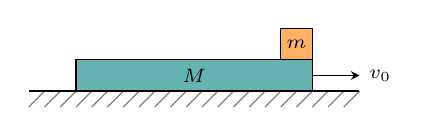
\begin{tikzpicture}[>=stealth,font=\scriptsize]
	\draw[fill=orange!60] (2.6,.4) rectangle(3,.8)node[midway]{\(m\)};
	\draw[fill=teal!60] (0,0) rectangle(3,.4)node[midway]{\(M\)};
	\draw[->] (3,.2)--++(.6,0)node[right]{\(v_0\)};
	\foreach \x in {-.6,-.4,...,3.6}
		\draw[gray] (\x,-.2)--++(.2,.2);
	\draw[thick] (-.6,0)--(3.6,0);
\end{tikzpicture}
\begin{choices}
	\item \(a_m =\) \,\qty{3}{m/s^2}
	\item \(a_M =\) \,\qty{2.5}{m/s^2}
	\item \(a_m =\) \,\qty{2}{m/s^2}
	\item \(a_M =\) \,\qty{3}{m/s^2}
\end{choices}
\begin{answer}
	C\qquad 提示：
\end{answer}